\documentclass[12pt]{scrreprt}
\usepackage[ngerman]{babel}

\usepackage[a4paper,left=4cm,right=2cm,top=2cm,bottom=2cm]{geometry}
\usepackage[utf8]{inputenc}
\usepackage{textcomp}
\DeclareUnicodeCharacter{0308}{\"}
\usepackage{enumitem}

%für Tabellenformation
\usepackage{pdflscape}
\usepackage{longtable} % Für Tabellen, die über eine Seite gehen
\usepackage{booktabs}  % Für schönere Tabellenlinien
\usepackage{ragged2e}  % Für besseren Textumbruch in Tabellen
\usepackage{array}

\usepackage{graphicx}
\usepackage{float}
\usepackage{caption}

%\usepackage[backend=biber, defernumbers=true]{biblatex} %Imports biblatex package
\usepackage{csquotes}
\usepackage{listings}
\usepackage[onehalfspacing]{setspace}
\usepackage{amsmath}
\usepackage{url}
\setlength{\parindent}{0pt}

\lstset{
	language=Java,
	basicstyle=\ttfamily\small,% Schriftgröße 10pt, Baselineskip 12pt
	keywordstyle=\ttfamily\small,
	stringstyle=\ttfamily\small,
	numbers = left,
	frame = single,
	breaklines=true
}

%\raggedbottom
\begin{document}
	
	\begin{titlepage}
		\centering
		
		
		\large
		Duale Hochschule Sachsen \\
		Staatliche Studienakademie Leipzig
		
		\vspace{2cm} 
		
		{\huge\bfseries Vergleich eines kommerziellen Intrusion-Prevention Systems und einer Open-Source-Lösung\par}
		
		\vspace{1.5cm} % Abstand
		

		{\Large Bachelorthesis\par}
		
		\vspace{0.5cm}
		

		zur Erlangung der staatlichen Abschlussbezeichnung eines \\
		Bachelor of Science (B. Sc.)
		
		\vspace{0.5cm} 
		
		im Studiengang Informatik
		
		\vfill 
		
		% --- Angaben zur Person und Gutachtern ---
		\begin{flushleft}
			\begin{tabular}{@{}ll}
				\textbf{Eingereicht von:} & Leon Baumgarten\\
				& Traupitzer Dorfstraße 23, 06729 Elsteraue \\
				& CS22-1 \\
				& 5002213 \\
				\\ 
				\textbf{Erstgutachter:} & B.Sc. Oliver Hels \\
				& WBS IT-Service GmbH\\
				\\ 
				\textbf{Zweitgutachter:} & Diplom IT Carsten Nitsch \\
				& Duale Hochschule Sachsen
			\end{tabular}
			
			\vspace{2cm}
			
{\today\par}
			
		\end{flushleft}
		
	\end{titlepage}
	
	
%	\begin{titlepage}
	%	\centering
	%	{\scshape\Large Duale Hochschule Leipzig \par}
	%	\vspace{1cm}
	%	{\scshape\Large Studiengang Informatik\linebreak Studienrichtung Informatik \par}
	%	\vspace{1.5cm}
	%	{\huge\bfseries Vergleich eines kommerziellen Intrusion-Prevention-Systems und einer Open-Source-Lösung\par}
	%	\vspace{2cm}
	%	{\large  Eingereicht von: \ Leon Baumgarten \linebreak 5CS22-1 \linebreak Matrikelnummer: 5002213 \par}
		
	%	\vfill
		
	%	{\large \today\par}
%	\end{titlepage} 
	\thispagestyle{empty}
	
	\tableofcontents
	\newpage
	
	\setcounter{page}{1}
	
	

	\chapter{Einleitung}

\section{Motivation und Problemstellung}
Die Digitalisierung durchdringt unaufhaltsam alle Bereiche von Wirtschaft und Gesellschaft. Während sie Effizienzgewinne, neue Geschäftsmodelle und eine globale Vernetzung ermöglicht, schafft sie gleichzeitig eine ebenso wachsende wie komplexe Angriffsfläche für Kriminalität. Die Bedrohungslage im Cyberraum hat sich in den letzten Jahren dramatisch verschärft und ist von einer Randnotiz für IT-Spezialisten zu einer strategischen Herausforderung für Unternehmen jeder Größenordnung geworden. Das Bundesamt für Sicherheit in der Informationstechnik (BSI) bewertet die Lage in seinem jährlichen Bericht als „angespannt bis besorgniserregend“ und verweist auf eine zunehmende Professionalisierung und Arbeitsteilung in der cyberkriminellen Schattenwirtschaft . \cite{BSI1}
\\\\
Die Angriffsvektoren sind vielfältig und reichen von Denial-of-Service-Angriffen (DoS), die gezielt die Nichtverfügbarkeit von Diensten herbeiführen, über die Infiltration von Netzwerken mittels Schadsoftware (Malware) wie Viren und Trojanern, bis hin zur aktiven Ausnutzung von Software-Schwachstellen durch Exploits. Insbesondere Ransomware-Angriffe, bei denen Daten verschlüsselt und nur gegen Lösegeld wieder freigegeben werden, haben sich zu einer der größten Bedrohungen für die deutsche Wirtschaft entwickelt. Laut einer Studie des Digitalverbands Bitkom entstanden hierdurch allein im Jahr 2024 Schäden in einer Höhe von 266,6 Milliarden Euro, wobei ein Großteil der Angriffe auf kleine und mittelständische Unternehmen (KMU) zielte. \cite{bitkom1}
\\\\
Gerade KMU stehen vor einer besonderen Herausforderung: Sie verfügen oft nicht über die gleichen finanziellen und personellen Ressourcen wie Großkonzerne, um sich umfassend zu schützen. Gleichzeitig sind sie aufgrund ihrer Rolle in Lieferketten und als Träger der regionalen Wirtschaft ein attraktives Ziel. Der traditionelle Schutz des Unternehmensnetzwerks durch eine reine Paketfilter-Firewall, die den Verkehr nur anhand von Ports und IP-Adressen kontrolliert, ist angesichts der modernen Bedrohungslage nicht mehr ausreichend. Angriffe finden heute oft auf der Anwendungsebene statt und verstecken sich im legitimen Datenverkehr, beispielsweise über den standardmäßigen Web-Port 443.
\\\\
An dieser Stelle setzen Intrusion Prevention Systeme (IPS) an. Als Weiterentwicklung von Intrusion Detection Systemen (IDS), die Angriffe nur erkennen und melden, sind IPS in der Lage, bösartigen Datenverkehr aktiv zu analysieren, zu klassifizieren und in Echtzeit zu blockieren, bevor er Schaden im internen Netzwerk anrichten kann. Diese Systeme agieren als wachsame "Torwächter", die den Inhalt der Datenpakete tiefgehend inspizieren (Deep Packet Inspection) und mit bekannten Angriffsmustern (Signaturen) oder anormalem Verhalten abgleichen.
\\\\
Für Unternehmen, die eine solche Schutztechnologie implementieren möchten, stellt sich eine grundlegende strategische Frage: Soll auf eine kommerzielle „All-in-One“-Lösung eines etablierten Herstellers gesetzt werden, oder kann eine flexiblere und potenziell kostengünstigere Open-Source-Lösung einen vergleichbaren Schutz bieten? Kommerzielle Produkte, oft als Next-Generation Firewalls (NGFW) vermarktet, versprechen eine hohe Integration, professionellen Support und eine einfache Verwaltung aus einer Hand. Demgegenüber stehen Open-Source-Alternativen, die durch Transparenz, Anpassbarkeit und den Wegfall von Lizenzgebühren überzeugen, jedoch oft ein höheres Maß an technischem Know-how in der Implementierung und Wartung erfordern.\\\\

Zusätzlich zu diesen externen Bedrohungen hat sich die Erkenntnis durchgesetzt, dass das interne Netzwerk (LAN) nicht per se als vertrauenswürdig gelten kann. Angriffe können ebenso von innen heraus erfolgen, sei es durch kompromittierte Endgeräte, die bereits Teil des Netzwerks sind, oder durch böswillige Insider. Dieses Paradigma, bekannt als Zero Trust, geht davon aus, dass Bedrohungen überall lauern können und somit auch der Datenverkehr innerhalb des Netzwerks einer Überprüfung bedarf. Eine zentrale Aufgabe moderner IPS ist es daher nicht mehr nur, die Grenze zum Internet zu schützen, sondern auch eine Segmentierung und Überwachung des internen Datenverkehrs zu ermöglichen.
\section{Stand der Technik und Forschungslücke}

Die vorliegende Arbeit positioniert sich exakt in diesem Spannungsfeld. Sie zielt darauf ab, den in der Praxis relevanten Entscheidungsprozess zwischen einem kommerziellen und einem Open-Source-System durch einen systematischen, technischen und praktischen Vergleich zu objektivieren.
\\\\
Als Repräsentant für die kommerzielle Welt wird eine FortiGate 70F der Firma Fortinet herangezogen. Fortinet ist einer der weltweiten Marktführer im Bereich der Netzwerksicherheit. Die FortiGate-Serie integriert Firewall-, VPN-, und IPS-Funktionen in einer einzigen Hardware-Appliance, die durch den Einsatz spezialisierter Security Processors (SPs) eine hohe Performance verspricht. Die 
\\\\
Als Gegenstück wird OPNsense untersucht, eine weit verbreitete und aktiv weiterentwickelte Open-Source-Firewall-Distribution, die auf dem robusten Betriebssystem FreeBSD basiert. OPNsense kann auf Standard-Hardware betrieben werden und integriert für die IPS-Funktionalität das leistungsfähige Open-Source-Engine Suricata. Suricata ist ein hochperformantes IDS/IPS, das von der Open Information Security Foundation (OISF) entwickelt wird. Im Gegensatz zum kommerziellen Ansatz ist der Anwender hier selbst dafür verantwortlich, die Hardware zu dimensionieren und die Regelwerke (Signaturen) aus verschiedenen freien oder auch kostenpflichtigen Quellen zu beziehen und zu verwalten.
\\\\
Während es zahlreiche Marketing-Vergleiche und allgemeine Gegenüberstellungen von Vor- und Nachteilen beider Ansätze gibt, fehlt es an detaillierten, praxisorientierten und reproduzierbaren Vergleichsstudien. Oft bleiben solche Analysen an der Oberfläche und vergleichen lediglich Feature-Listen, ohne die tatsächliche Schutzwirkung und die betrieblichen Aspekte in einer kontrollierten Umgebung zu testen. Diese Arbeit schließt diese Lücke, indem sie nicht nur die theoretischen Konzepte, sondern die konkrete Implementierung und Leistungsfähigkeit von FortiGate und OPNsense in einem eigens aufgebauten Testlabor direkt gegenüberstellt.

\section{Zielsetzung und Forschungsfragen}

Das primäre Ziel dieser Bachelorarbeit ist es, eine fundierte und objektive Entscheidungsgrundlage vor allem für KMU zu schaffen, die vor der Wahl eines geeigneten IPS stehen. Es soll ermittelt werden, inwieweit die Open-Source-Lösung OPNsense eine technisch ebenbürtige und praktikable Alternative zum kommerziellen Marktführer FortiGate darstellt.\\

\textbf{Um dieses Ziel zu erreichen, wird die Untersuchung von folgender zentraler Forschungsfrage geleitet:}\\

Inwieweit kann das Open-Source-System OPNsense in Bezug auf Schutzwirkung, Performance und Verwaltungsaufwand eine effektive Alternative zur kommerziellen Next-Generation-Firewall FortiGate für den Einsatz in kleinen und mittelständischen Unternehmen darstellen?\\

\textbf{Zur systematischen Beantwortung dieser Hauptfrage werden die folgenden untergeordneten Forschungsfragen untersucht:}\\

Worin liegen die konzeptionellen und architektonischen Unterschiede bei der Implementierung der IPS-Funktionalität in der FortiGate-Appliance und dem OPNsense-System mit Suricata?\\

Wie effektiv erkennen und blockieren beide Systeme eine Reihe definierter, praxisnaher Angriffe aus den Kategorien Malware, Exploits und Denial-of-Service in einer kontrollierten Testumgebung?\\

Welche qualitativen Unterschiede bestehen hinsichtlich des Konfigurationsaufwands, der Benutzerfreundlichkeit der Verwaltungsoberflächen und der Qualität der Protokollierungs- und Reporting-Funktionen?\\

Welche quantifizierbaren Auswirkungen hat die Aktivierung der IPS-Funktionen auf den Netzwerkdurchsatz und die Latenz bei beiden Systemen?

\section{Aufbau der Arbeit}

Die Struktur der vorliegenden Arbeit orientiert sich konsequent an der Beantwortung der formulierten Forschungsfragen.\\

Das erste Kapitel legt die theoretischen Grundlagen. Es wird ein Überblick über die aktuelle Bedrohungslage gegeben und die Funktionsweise sowie die technologischen Konzepte von Intrusion Detection- und Prevention Systemen erläutert. Anschließend werden die beiden zu vergleichenden Systeme, FortiGate und OPNsense, mit ihren jeweiligen Architekturen und Besonderheiten vorgestellt.\\

Im zweiten Kapitel wird der Aufbau der Testumgebung detailliert beschrieben. Dies umfasst die Auswahl der Hardware- und Softwarekomponenten, die entworfene Netzwerkarchitektur sowie die grundlegende Konfiguration der beiden IPS-Systeme, um eine transparente und nachvollziehbare Testbasis zu schaffen.\\

Das dritte Kapitel widmet sich dem Testing. Hier werden die konkreten Testfälle, die zur Überprüfung der Schutzwirkung und Performance dienen, definiert und deren Durchführung systematisch protokolliert.\\

Die im Praxisteil gewonnenen Daten werden im vierten Kapitel ausgewertet. Zunächst werden die Testergebnisse analysiert und anschließend die beiden Systeme anhand der zuvor definierten Kriterien wie Erkennungsrate, Performance und Benutzerfreundlichkeit verglichen. \\

Das fünfte und letzte Kapitel fasst die Erkenntnisse in einem Fazit zusammen, beantwortet die Forschungsfragen und gibt eine abschließende Bewertung sowie eine Handlungsempfehlung ab. 
	
	\chapter{Theoretische Grundlagen}

\section{Bedrohungslage}
Die Kernaufgabe eines jeden technischen Sicherheitssystems, insbesondere eines Intrusion Prevention Systems (IPS), ist die Erkennung und Abwehr konkreter Angriffe. Eine systematische Analyse und ein aussagekräftiger Vergleich solcher Systeme, wie er in dieser Arbeit angestrebt wird, setzen daher zwingend ein klares Verständnis der zu bekämpfenden Bedrohungen voraus.\\

 Bevor die Fähigkeiten der Testsysteme praktisch evaluiert werden können, muss dieses theoretische Fundament geschaffen werden. Aus diesem Grund konzentriert sich dieser Abschnitt auf drei fundamentale Angriffskategorien, die für die Prüfung eines IPS zentral sind: Denial-of-Service-Angriffe, die Infiltration durch Malware und die Ausnutzung von Exploits. \\
  Die nachfolgenden Unterkapitel widmen sich jeweils einer dieser Kategorien. Es werden die technischen Grundlagen, gängige Varianten und die charakteristischen Merkmale erläutert, anhand derer ein Schutzsystem den jeweiligen Angriff erkennen kann. Dieses Wissen ist die Voraussetzung, um die Konfiguration der Systeme im Testaufbau nachzuvollziehen und die Ergebnisse der praktischen Tests zu analysieren. \cite{cloudflare1}
  
  
\subsection{Denial-of-Service-Angriff}

Ein Denial-of-Service-Angriff (DoS), oder in seiner heute weitaus verbreiteteren Form als Distributed-Denial-of-Service-Angriff (DDoS), zielt fundamental auf die Beeinträchtigung der Verfügbarkeit eines IT-Dienstes ab. Das Ziel ist die Sabotage des regulären Betriebs, indem die endlichen Ressourcen des Zielsystems gezielt erschöpft werden. Bei einem DDoS-Angriff wird diese Überlastung durch eine Vielzahl kompromittierter Systeme, einem sogenannten Botnetz, gleichzeitig herbeigeführt. Diese massive Parallelisierung macht eine simple Abwehr durch das Blockieren einzelner IP-Adressen praktisch unmöglich.\\

Technisch lassen sich diese Angriffe in drei Hauptkategorien unterteilen, die auf unterschiedliche Schichten des OSI-Modells abzielen:\\

\textbf{Volumetrische Angriffe (Schicht 3/4):} Diese Angriffe zielen darauf ab, die gesamte zur Verfügung stehende Netzwerkbandbreite der Internetanbindung des Ziels zu sättigen. Eine Flut von Paketen wird an ein Ziel gerichtet. Ein klassisches Beispiel ist der UDP-Flood, bei dem eine riesige Menge an UDP-Paketen an zufällige Ports des Zielsystems gesendet wird. Da UDP ein verbindungsloses Protokoll ist, muss der Server für jedes eingehende Paket prüfen, ob eine Anwendung auf dem Port lauscht, und eine ICMP-Antwort "Destination Unreachable" generieren, was seine Ressourcen bindet. Ein ICMP-Flood (oder Ping-Flood) funktioniert nach einem ähnlichen Prinzip, indem er das Ziel mit ICMP-Echo-Request-Paketen überflutet und es zwingt, eine ebenso große Anzahl von Echo-Reply-Paketen zu senden. Das primäre Ziel ist hier die reine Masse an Traffic. \\

\textbf{Protokoll-Angriffe (Schicht 4):} Diese Angriffe nutzen Schwachstellen in der Implementierung von Netzwerkprotokollen aus, um die Ressourcen von Netzwerkkomponenten wie Firewalls oder Load Balancern zu erschöpfen. Der bekannteste Vertreter ist der TCP-SYN-Flood. Er missbraucht den drei-Wege-Handshake von TCP (SYN, SYN-ACK, ACK). Der Angreifer sendet eine hohe Zahl von SYN-Paketen, oft von gefälschten Quell-IP-Adressen. Das Zielsystem antwortet mit SYN-ACK und reserviert Ressourcen in seiner Verbindungstabelle (Backlog Queue) für die erwartete ACK-Antwort. Da diese Antwort niemals eintrifft, bleiben die Verbindungen "halboffen", bis die Tabelle voll ist und keine neuen, legitimen Verbindungsanfragen mehr angenommen werden können und überlastet ist. \\

\textbf{Angriffe auf der Anwendungsebene (Schicht 7):} Diese Angriffe sind subtiler und oft schwerer zu erkennen, da sie scheinbar legitimen Traffic imitieren. Sie zielen nicht auf die Netzwerkbandbreite, sondern auf die CPU- und Speicherressourcen des Servers ab. Beispiele hierfür sind das wiederholte Anfordern sehr großer Dateien oder das Ausführen komplexer Suchanfragen über eine Website, die serverseitig aufwändige Datenbankoperationen auslösen. Auch Angriffe auf Login-Schnittstellen durch massenhafte POST-Requests oder das Ausnutzen rechenintensiver API-Endpunkte fallen in diese Kategorie. Da diese Angriffe oft mit einer relativ geringen Datenrate auskommen, können sie unter dem Radar traditioneller, rein volumetrisch arbeitender Schutzsysteme hindurchgehen.\\ \cite{cloudflare1,rfc1} 

Für ein Intrusion Prevention System besteht die Herausforderung darin, die Muster dieser unterschiedlichen Angriffsarten von legitimen Lastspitzen zu unterscheiden und sie präzise zu blockieren, ohne den regulären Nutzerverkehr zu beeinträchtigen.

\subsection{Malware}

Der Begriff Malware, eine Kurzform für "malicious software", dient als Oberbegriff für jegliche Art von Software, die mit der Absicht entwickelt wurde, auf einem Computersystem unerwünschte oder schädliche Aktionen auszuführen, Daten zu entwenden oder unautorisierten Zugriff zu erlangen. Die Ziele sind dabei vielfältig und reichen vom Diebstahl sensibler persönlicher oder geschäftlicher Informationen über die Störung von Betriebsabläufen, bis hin zur vollständigen Übernahme der Kontrolle über ein System, um es beispielsweise als Teil eines Botnetzes für DDoS-Angriffe zu missbrauchen. Die Infektion eines Netzwerks erfolgt oft mit einem mehrstufigen Prozess.\\

 Zuerst muss die Malware auf das Zielsystem gelangen (Zustellung), was meist durch das Öffnen von manipulierten E-Mail-Anhängen (Phishing), das Klicken auf Links zu kompromittierten Websites (Drive-by-Downloads) oder über infizierte externe Speichermedien geschieht. Anschließend wird die Malware durch eine Benutzerinteraktion oder eine Sicherheitslücke aktiviert (Ausführung) und installiert sich fest im System, um einen Neustart zu überdauern (Persistenz). In vielen Fällen kontaktiert die Schadsoftware danach einen externen Command-and-Control-Server des Angreifers, um Anweisungen zu empfangen oder gestohlene Daten zu übermitteln.\\

Je nach Vorgehensweise und primärer Funktion lässt sich Malware in verschiedene Haupttypen klassifizieren, deren Grenzen jedoch zunehmend verschwimmen. Eine grundlegende Unterscheidung ist für das Verständnis der Bedrohungslandschaft unerlässlich.\\

\textbf{Viren:}\\
Klassische Viren sind Programmsegmente, die sich nicht eigenständig ausführen können, sondern eine legitime, ausführbare Wirtsdatei benötigen, um sich zu verbreiten. Sobald der Nutzer diese infizierte Datei startet, wird auch der virale Code aktiviert, der sich dann in weitere Dateien auf dem System oder auf verbundenen Netzlaufwerken kopiert. Die Schadfunktion, die von der reinen Replikation bis zur Zerstörung von Daten reichen kann, wird erst durch diese Nutzerinteraktion ausgelöst.\cite{BSI1} \\

\textbf{Würmer:}\\
Im Gegensatz dazu sind Würmer eigenständige Schadprogramme, die sich aktiv und ohne Zutun des Nutzers über Netzwerke verbreiten. Sie nutzen gezielt Sicherheitslücken in Betriebssystemen oder Anwendungen aus, um sich von einem infizierten System auf andere, verwundbare Systeme zu replizieren. Dieser autonome Verbreitungsmechanismus kann zu einer extrem schnellen, kaskadenartigen Infektionswelle führen, die ganze Unternehmensnetzwerke lahmlegt. Ein prominentes Beispiel hierfür ist der Wurm WannaCry, der 2017 die ''EternalBlue''-Schwachstelle im SMB-Protokoll von Windows-Systemen ausnutzte, um sich weltweit zu verbreiten und auf den infizierten Systemen Ransomware zu installieren.\cite{BSI12} \\

\textbf{Trojaner:}\\
Trojaner, benannt in Anlehnung an das Trojanische Pferd der griechischen Mythologie, tarnen sich als nützliche oder legitime Software, um den Nutzer zur Installation zu bewegen. Sie enthalten jedoch eine versteckte, bösartige Funktion. Nach der Ausführung installieren sie oft eine Hintertür (Backdoor), die Angreifern einen permanenten und unbemerkten Fernzugriff auf das System ermöglicht. Solche Remote Access Trojans (RATs) erlauben es Angreifern, Daten zu stehlen, das System zu überwachen oder es als Teil eines Botnetzes für weitere Angriffe zu missbrauchen.\cite{kasp1}\\

\textbf{Ransomware:}\\
Eine besonders profitable und schädliche Form ist die Ransomware. Diese Malware verschlüsselt die Dateien des Opfers, sodass auf sie nicht mehr zugegriffen werden kann. Anschließend wird eine Lösegeldforderung angezeigt, meist zahlbar in Kryptowährungen, um die Anonymität der Täter zu wahren. In den letzten Jahren hat sich das Vorgehen zur sogenannten "Double Extortion" (doppelte Erpressung) weiterentwickelt. Hierbei werden die Daten vor der Verschlüsselung zusätzlich vom System des Opfers auf Server der Angreifer kopiert. Wird das Lösegeld nicht gezahlt, drohen die Täter nicht nur mit der permanenten Zerstörung der Daten, sondern auch mit deren Veröffentlichung.\cite{ENISA1}\\

\textbf{Spyware:}\\
Davon abzugrenzen ist Spyware, deren Hauptziel es ist, verdeckt Informationen über den Nutzer, dessen Verhalten und die auf dem System gespeicherten Daten zu sammeln. Eine der bekanntesten Unterarten sind Keylogger, die jeden Tastaturanschlag protokollieren. Auf diese Weise können Angreifer sensible Informationen wie Passwörter, Kreditkartennummern oder private Nachrichten mitschneiden und an ihre Server übermitteln.\\

Durch die Analyse von bekannten Malware-Signaturen, das Erkennen von Anomalien im Protokollverfahren und das Blockieren von Verbindungen zu IP-Adressen und Domains können IPS-Systeme diese Bedrohungen erkennen und unterbinden.



\subsection{Exploits}
Der Begriff Exploit bezeichnet ein spezifisches Software-Fragment, einen Datenblock oder eine Befehlssequenz, die gezielt einen Programmierfehler oder eine konzeptionelle Schwachstelle in einem Computersystem oder einer Anwendung ausnutzt. Es ist entscheidend, zwischen der Schwachstelle, bei der es sich um einen passiven, latenten Fehler im Code handelt, und dem Exploit, dem aktiven Werkzeug zur Ausnutzung dieses Fehlers, zu unterscheiden. Das Ziel eines Exploits ist es, erhöhte Rechte zu erlangen (Privilege Escalation), beliebigen Code auf dem Zielsystem auszuführen (Arbitrary Code Execution) oder einen Denial-of-Service-Zustand auszulösen. Dies macht Exploits zu einem primären Vektor für den erstmaligen Einbruch in ein Netzwerk.\cite{wik12}\\

Der Prozess eines Angriffs, der auf der Ausnutzung von Schwachstellen basiert, lässt sich in die sieben Phasen der Cyber Kill Chain unterteilen, die den Ablauf aus der Perspektive des Angreifers strukturieren. Die erste Phase ist die \textbf{Reconnaissance}, in der ein Angreifer Informationen über das Ziel sammelt, um potenzielle Angriffsvektoren zu finden. In der zweiten Phase, der \textbf{Weaponization}, wird ein passender Exploit-Code mit einer Nutzlast (Payload) – dem eigentlichen Schadcode – gekoppelt. Anschließend erfolgt die \textbf{Delivery}, bei der der vorbereitete Exploit an das Zielsystem übermittelt wird, beispielsweise über eine Phishing-Mail oder einen verwundbaren Netzwerkdienst.\\

In der vierten Phase, der \textbf{Exploitation}, wird der Exploit-Code zur Ausführung gebracht und löst den Fehler in der verwundbaren Software aus. Dies ermöglicht die Ausführung des mitgelieferten Payload. Darauf folgt die \textbf{Installation}, in der die Payload Persistenz auf dem System etabliert, um nach einem Neustart noch auf dem Zielsystem vorhanden zu sein. In der sechsten Phase, \textbf{Command and Control} (C2), baut die installierte Schadsoftware eine ausgehende Verbindung zu einem vom Angreifer kontrollierten Server auf. Über diesen Kanal kann der Angreifer das System fernsteuern. In der letzten Phase, \textbf{Actions on Objectives}, verfolgt der Angreifer seine eigentlichen Ziele, wie zum Beispiel den Diebstahl von Daten, die Ausbreitung im internen Netzwerk, oder die Verschlüsselung von Systemen zur Erpressung von Lösegeld.\cite{wik1}\\

\textbf{Zero-Day-Exploit:}\\
Die gefährlichste Kategorie sind Zero-Day-Exploits. Der Begriff „Zero-Day“ leitet sich aus der Perspektive des Softwareherstellers ab: Ab dem Moment, in dem ein Exploit für eine bisher unbekannte Schwachstelle aktiv ausgenutzt wird, hat der Hersteller null Tage Zeit gehabt, einen entsprechenden Sicherheitspatch zu entwickeln und bereitzustellen. Diese Unkenntnis aufseiten der Verteidiger verschafft den Angreifern ein kritisches Zeitfenster, in dem ihre Angriffe mit sehr hoher Wahrscheinlichkeit erfolgreich sind.\\
Die besondere Gefahr von Zero-Day-Exploits liegt in ihrer Fähigkeit, traditionelle, signaturbasierte Schutzmechanismen wie die meisten Antivirenprogramme und Intrusion Prevention Systeme vollständig zu umgehen. Da der Angriff neu und unbekannt ist, existiert keine Signatur, kein Muster und kein Hashwert, nach dem ein solches System suchen könnte. Der Exploit ist für die Verteidigungslinie demnach quasi unsichtbar.\\
Die Abwehr von Zero-Day-Angriffen erfordert daher fortschrittlichere Sicherheitsstrategien, die über die reine Signaturerkennung hinausgehen. Dazu gehören verhaltensbasierte Analyse (Heuristik) und Anomalieerkennung, bei denen ein System nicht nach bekannten Mustern, sondern nach ungewöhnlichem und potenziell bösartigem Verhalten sucht. Eine weitere wichtige Technik ist das Sandboxing, bei dem verdächtiger Code in einer isolierten, virtuellen Umgebung ausgeführt wird, um seine Aktionen zu beobachten, ohne das eigentliche System zu gefährden.

\section{IDS / IPS Grundlagen}
Nach der detaillierten Betrachtung der vielfältigen Bedrohungslandschaft im vorherigen Kapitel, werden nun die Systeme näher beleuchtet, die entwickelt wurden, um Netzwerke vor genannten Angriffen zu schützen. Während klassische Firewalls den Verkehr primär anhand von Adressen und Ports (Schicht 3 und 4 des OSI-Modells) filtern, gehen moderne Schutzmechanismen einen entscheidenden Schritt weiter, indem sie den Inhalt des Datenverkehrs analysieren. Im Zentrum dieser erweiterten Sicherheitsarchitektur stehen Intrusion Detection- und Intrusion Prevention-Systeme (IDS/IPS).

In den folgenden Absätzen werden dazu die theoretischen Grundlagen dieser Technologien erklärt. Es wird die evolutionäre Entwicklung vom rein passiven Erkennen eines Angriffs (Detection) hin zum aktiven Verhindern (Prevention) nachgezeichnet, um die grundlegenden Unterschiede und die Motivation hinter der Entwicklung von IPS zu beleuchten. Anschließend wird das technische Funktionsprinzip der Deep Packet Inspection (DPI) erläutert, das es diesen Systemen überhaupt erst ermöglicht, den Inhalt von Datenpaketen zu analysieren. Abschließend folgt die Vorstellung der verschiedenen Erkennungsmethoden, auf deren Basis ein System die Entscheidung trifft, ob es sich um legitimen oder bösartigen Datenverkehr handelt.

\subsection{Vom passiven Detektieren zum aktiven Verhindern}

Die historischen Vorläufer moderner Angriffserkennungssysteme sind die Intrusion Detection Systeme (IDS). Sie entstanden aus der Notwendigkeit heraus, die Sicherheitsarchitekturen von Netzwerken zu ergänzen, da klassische Paketfilter-Firewalls allein nicht mehr ausreichten, um Angriffe auf höheren Protokollebenen zu erkennen. Das grundlegende Funktionsprinzip eines netzwerkbasierten IDS (NIDS) ist die der passiven Überwachung. Ein IDS wird im Netzwerk so implementiert, dass es eine Kopie des gesamten zu überwachenden Datenverkehrs erhält, ohne selbst Teil des aktiven Datenpfades zu sein. Technisch wird dies meist über einen sogenannten Mirror-Port (auch SPAN-Port genannt) an einem Netzwerk-Switch realisiert, der den gesamten Verkehr eines oder mehrerer anderer Ports auf den Port des IDS spiegelt. Eine alternative, oft als zuverlässiger geltende Methode ist der Einsatz eines dedizierten Network Taps, einer Hardware-Komponente, die direkt in die Leitung eingeschleift wird und eine verlustfreie Kopie des Verkehrs auskoppelt. Unabhängig von der Methode agiert das IDS somit stets wie ein Beobachter, der den Verkehr analysiert, ihn jedoch nicht direkt beeinflusst. Stellt das System eine potenzielle Bedrohung fest, ist seine primäre Aufgabe das Auslösen eines Alarms. Dieser Alarm kann in Form eines Eintrags in einer Log-Datei, einer Benachrichtigung per E-Mail oder einer Meldung an ein übergeordnetes Security Information and Event Management (SIEM) System erfolgen, wo die Daten für eine weitere Analyse korreliert werden. Die Kernfunktion eines IDS ist also die reine Detektion; es beantwortet die Frage: „Passiert hier gerade etwas Bösartiges?“ \cite{Claudia1}.\\

\textbf{Definition Network Tap:}\\
Ein Network TAP (Test Access Point) ist eine dedizierte Hardware-Komponente, die eine exakte, verlustfreie Kopie des gesamten Datenverkehrs von einer physischen Netzwerkverbindung erstellt. Das Gerät wird direkt in die Kabelverbindung, beispielsweise zwischen einem Router und einem Switch, eingeschleift und leitet den durchfließenden Verkehr passiv an einen oder mehrere Monitor-Ports weiter, an denen das Überwachungssystem angeschlossen ist. Im Gegensatz zu einem SPAN-Port eines Switches, der bei hoher Netzwerkauslastung unter Umständen Pakete verwirft, garantiert ein TAP die Weiterleitung allen Traffics, einschließlich fehlerhafter Pakete. Zudem sind die meisten TAPs ausfallsicher konzipiert.\cite{TAP1}\\

Die entscheidende Schwäche dieses passiven Ansatzes liegt in der systembedingten Latenz zwischen der Erkennung eines Angriffs und der Einleitung einer Gegenmaßnahme. Nachdem ein IDS einen Alarm ausgelöst hat, ist eine Reaktion erforderlich, um den Angriff zu stoppen. Diese Reaktion kann manuell durch einen Administrator erfolgen, der beispielsweise eine neue Regel in der Firewall konfiguriert, oder durch ein nachgeschaltetes, automatisiertes System. In der Zeit, die dieser Prozess unweigerlich in Anspruch nimmt, kann der Angriff sein Ziel bereits erreicht und erheblichen Schaden verursacht haben. Ein weiteres gravierendes, operatives Problem ist die sogenannte „Alert Fatigue“ (Alarm-Müdigkeit). Hochsensibel konfigurierte IDS können eine enorme Menge an Alarmen generieren, von denen viele Falschmeldungen (False Positives) sind. Administratoren werden von dieser Flut an Informationen überfordert, was dazu führen kann, dass sie kritische, echte Alarme übersehen oder weniger ernst nehmen.\\

Um diese kritische Schutzlücke zu schließen und die Reaktionszeit auf null zu reduzieren, wurden die Intrusion Prevention Systeme (IPS) entwickelt. Im Gegensatz zu einem IDS wird ein IPS aktiv und „in-line“ im Netzwerk platziert und behebt damit dessen grundlegende Schwäche. Diese architektonische Entscheidung ist fundamental: Das IPS fungiert als aktiver Kontrollpunkt, den der gesamte Datenverkehr passieren muss, um sein Ziel zu erreichen. Dies birgt jedoch auch neue Risiken: Ein IPS kann zu einem Leistungsengpass (Bottleneck) werden und stellt einen Single Point of Failure dar. Fällt das IPS aus, wird die gesamte Netzwerkverbindung unterbrochen, sofern keine Bypass-Mechanismen vorhanden sind.\\

Diese direkte Positionierung im Datenstrom ermöglicht es einem IPS, nicht nur zu erkennen, sondern auch unmittelbar und automatisiert zu handeln. Erkennt es einen Angriff, kann es eine Reihe von vordefinierten Aktionen durchführen. Die Palette dieser Reaktionsmöglichkeiten ist breit und reicht von dem einfachen Blockieren oder Verwerfen (Block/Drop) einzelner bösartiger Datenpakete über das aktive Zurücksetzen von TCP-Verbindungen (Reset), um eine Sitzung sauber zu beenden, bis hin zur reinen Alarmierung (Alert). Letztere wird genutzt, um neue Regeln im Überwachungsmodus zu testen, ohne den produktiven Verkehr zu gefährden. \cite{Suricata1, NIST1}\\

Darüber hinaus bieten viele Systeme erweiterte, oftmals herstellerabhängige Reaktionsmöglichkeiten. Dazu zählt beispielsweise die temporäre Sperrung der angreifenden IP-Adresse (Shun) oder die Umleitung des Angriffsverkehrs auf ein Ködersystem (Quarantäne/Sinkhole) zur weiteren Analyse und zur Sammlung von Informationen über den Angreifer. Die genaue Auswahl und die Granularität der verfügbaren Aktionen sind ein wesentliches Unterscheidungsmerkmal des jeweiligen Produkts und ein Indikator für seine technische Reife. Welche dieser Funktionen von den in dieser Arbeit untersuchten Systemen, FortiGate und OPNsense, im Detail unterstützt werden, wird im Rahmen ihrer jeweiligen Vorstellung in Kapitel 2.3 detailliert erläutert.
\newpage
\subsection{Funktionsprinzip: Deep Packet Inspection (DPI)}
Die technologische Grundlage, die moderne Intrusion Prevention Systeme von klassischen Firewalls unterscheidet und ihre Effektivität überhaupt erst ermöglicht, ist die Deep Packet Inspection (DPI). Während traditionelle Paketfilter ihre Entscheidungen ausschließlich auf Basis der Header-Informationen der Schichten 3 und 4 des OSI-Modells (IP-Adressen, Ports) treffen, geht die DPI-Technologie entscheidende Schritte weiter. Selbst die fortgeschrittenere Stateful Packet Inspection (SPI), die den Zustand von Verbindungen verfolgt, analysiert nicht den eigentlichen Inhalt der übertragenen Daten. Die DPI hingegen untersucht nicht nur die Header, sondern auch die Nutzlast (Payload) der Datenpakete und kann den Datenstrom bis zur Anwendungsschicht (Schicht 7) analysieren, um so den Kontext und die Bedeutung der übertragenen Daten zu verstehen.\\

Der Funktionsprozess einer DPI-Engine ist hochkomplex und muss in Echtzeit ablaufen. Der erste Schritt in diesem Prozess ist die Paket-Normalisierung und Strom-Reassemblierung. Ein IPS empfängt den Netzwerkverkehr als eine Sequenz einzelner Datenpakete, die durch Fragmentierung oder durch die Netzwerkübertragung selbst in falscher Reihenfolge (Out-of-Order) eintreffen können. Die DPI-Engine muss diese Pakete daher anhand ihrer TCP-Sequenznummern korrekt sortieren und zu einem kohärenten, bidirektionalen Datenstrom zusammensetzen. Dieser Schritt ist kritisch, da viele Angriffstechniken gezielt versuchen, durch manipulierte Fragmentierung die Erkennung zu umgehen. Darauf aufbauend muss die Engine den reassemblierten Datenstrom dekodieren, um die genutzten Anwendungsprotokolle wie HTTP, SMB oder DNS zu identifizieren. Anschließend wird der Strom gemäß der Spezifikation des jeweiligen Protokolls geparst, also in seine logischen Bestandteile zerlegt, um zwischen Kontrollinformationen und der eigentlichen Nutzlast zu unterscheiden.\\

Im Kern der DPI steht dann die eigentliche Inhaltsanalyse. Nachdem die Daten durch die vorherigen Schritte aufbereitet und in ihren protokollspezifischen Kontext gebracht wurden, werden sie an die eigentliche Analyse-Engine des IPS weitergeleitet. Die Aufgabe dieser Engine ist es, den Inhalt der Nutzlast zu bewerten und eine Entscheidung über dessen Zulässigkeit zu treffen. Hierfür greift das System auf verschiedene logische Verfahren zurück, um bösartige von gutartigen Daten zu unterscheiden. Die genaue Funktionsweise dieser zentralen Erkennungsmethoden, insbesondere der signaturbasierten und der anomaliebasierten Analyse, wird im nachfolgenden Kapitel 2.2.3 detailliert erläutert.\\

Die größte technische Hürde stellt jedoch der zunehmend verschlüsselte Datenverkehr (SSL/TLS) dar. Um die Nutzlast von HTTPS-Verbindungen zu inspizieren, muss das IPS eine als SSL/TLS-Inspektion bekannte Methode anwenden und als autorisierter „Man-in-the-Middle“ agieren. Dabei fängt das IPS die Verbindungsanfrage des Clients ab, baut selbst eine Verbindung zum Zielserver auf und präsentiert dem Client ein eigenes zur Laufzeit generiertes Zertifikat. Damit dieser Prozess funktioniert, muss das Zertifikat der IPS-internen Certifikatsstelle auf allen Client-Systemen als vertrauenswürdig hinterlegt sein. Nur so kann das IPS den Verkehr transparent entschlüsseln, mit den beschriebenen Methoden analysieren und anschließend neu verschlüsselt zum Zielserver weiterleiten. Dieser Vorgang ist extrem rechenintensiv und verdeutlicht die Notwendigkeit spezialisierter Hardware in leistungsfähigen IPS-Systemen. Ohne die Fähigkeit der DPI, tief in die Nutzlast von Datenpaketen zu blicken, wäre ein Schutzsystem blind für nahezu alle modernen Angriffe auf der Anwendungsebene. \cite{NIST1,Claudia1}

\subsection{Zentrale Erkennungsmethoden}
Nachdem die Deep Packet Inspection (DPI) den Netzwerkverkehr in einen analysierbaren, reassemblierten Datenstrom umgewandelt hat, beginnt der eigentliche Analyseprozess. An dieser Stelle kommen die Erkennungs-Engines des IPS zum Einsatz, die auf zwei fundamentalen, konzeptionell unterschiedlichen Paradigmen basieren: der signaturbasierten Erkennung, die auch als Missbrauchserkennung (Misuse Detection) bekannt ist, und der anomaliebasierten Erkennung (Anomaly Detection). Diese beiden Methoden bilden das logische Herzstück eines jeden IPS.\\

\textbf{Signaturbasierte Erkennung:}

Die signaturbasierte Erkennung, auch als Missbrauchserkennung (Misuse Detection) bekannt, stellt den fundamentalen und historisch älteren Ansatz zur Identifizierung von Cyber-Angriffen dar. Sie basiert auf einem fest definierten, vorab erstellten Wissensschatz über bekannte Bedrohungen und sucht im Netzwerkverkehr exakt nach den Mustern, die diesen Bedrohungen zugeordnet sind. Das zugrundeliegende Prinzip ist vergleichbar mit dem eines Virenscanners, der nach den eindeutigen "Fingerabdrücken" bekannter Viren sucht, jedoch auf der Ebene von Netzwerkprotokollen und Datenströmen.\\

Der Lebenszyklus einer Signatur beginnt mit der Entdeckung einer neuen Bedrohung. Sicherheitsforscher bei Herstellern wie Fortinet oder in Open-Source-Communities analysieren neue Malware oder die Vorgehensweise eines Exploits im Detail. Dabei extrahieren sie eindeutige, unveränderliche Merkmale. Dies kann eine bestimmte Zeichenfolge in der Nutzlast, eine charakteristische Abfolge von Befehlen oder ein spezifischer Wert in einem Protokoll-Header sein. Auf Basis dieser Analyse wird eine Signatur als formale Regel erstellt. Eine moderne Signatur ist dabei weit mehr als eine simple Zeichenkette. Sie ist ein mehrdimensionales Konstrukt, das typischerweise folgende Elemente umfasst:\\
\setlist{noitemsep}
\begin{itemize}
	\item \textbf{Header-Bedingungen:} \\Diese legen den Geltungsbereich der Regel fest und filtern den zu untersuchenden Verkehr vor. Hierzu gehören Protokoll (TCP, UDP, ICMP), Quell- und Ziel-IP-Adressen (oder ganze Subnetze) sowie Port-Nummern.\\
	\item \textbf{Inhalts-Muster (Payload Content):} \\Der Kern der Signatur. Hier werden die eigentlichen bösartigen Muster definiert, oft als Byte-Sequenzen oder als flexible reguläre Ausdrücke.\\
	\item \textbf{Kontextuelle Optionen: } \\Diese verfeinern die Regel, um Falschmeldungen zu minimieren. So kann eine Regel beispielsweise festlegen, dass ein bestimmtes Muster nur dann als bösartig gilt, wenn es in einem HTTP-POST-Request an einen bestimmten URL-Pfad auftritt oder wenn es nicht von einer bestimmten anderen Zeichenfolge gefolgt wird.\\
	\item \textbf{Metadaten:} \\Jede Signatur wird mit zusätzlichen Informationen wie einer eindeutigen ID, einer Referenz zur entsprechenden CVE-Nummer (Common Vulnerabilities and Exposures), einer Beschreibung des Angriffs und einer Klassifizierung der Bedrohungsschwere versehen
\end{itemize}

Technisch werden zwei Arten von Signaturen unterschieden: atomare Signaturen, die ein einzelnes Paket auf ein Muster hin untersuchen, und zustandsbehaftete (stateful) Signaturen, die den Zustand einer gesamten Verbindung über mehrere Pakete hinweg verfolgen und erst dann anschlagen, wenn eine bestimmte Abfolge von Ereignissen eingetreten ist. Zustandsbehaftete Signaturen sind weitaus mächtiger, aber auch rechenintensiver. Um die immense Aufgabe zu bewältigen, Tausende dieser komplexen Regeln in Echtzeit auf einen Datenstrom mit Gigabit-Geschwindigkeit anzuwenden, werden die Signaturen beim Start des IPS in optimierte Datenstrukturen geladen. Dies ermöglicht einen simultanen Abgleich aller Muster in einem einzigen Durchlauf.\\

Der entscheidende Vorteil der signaturbasierten Erkennung liegt in ihrer hohen Präzision und Zuverlässigkeit. Ein positiver Treffer ist ein starker Indikator für einen tatsächlichen, bekannten Angriff, was die Rate an False Positives extrem niedrig hält. Die Nachteile sind jedoch ebenso nicht zu vernachlässigen. Die Methode ist per Definition reaktiv; sie kann einen Angriff erst erkennen, nachdem er analysiert und eine Signatur dafür erstellt und verteilt wurde. Gegen Zero-Day-Exploits ist sie daher wirkungslos. Zudem versuchen Angreifer gezielt, Signaturen durch Evasion-Techniken zu umgehen. Mittels Polymorphismus oder Metamorphismus wird der Schadcode bei jeder Infektion automatisch so verändert, dass sein "Fingerabdruck" variiert. Durch Verschleierung, beispielsweise durch Kodierung oder Verschlüsselung der Nutzlast, wird versucht, den bösartigen Inhalt vor der DPI-Engine zu verbergen. Die Effektivität eines signaturbasierten IPS hängt somit direkt und unabdingbar von der Qualität, der Geschwindigkeit und der Intelligenz der Signatur-Updates des jeweiligen Herstellers oder der Community ab.\\

\textbf{Anomaliebasierte Erkennung:}

Die anomaliebasierte Erkennung verfolgt einen fundamental anderen, induktiven Ansatz. Statt nach bekannten Mustern des ''Bösen'' zu suchen, versucht sie, ein umfassendes Modell des ''Normalen'' zu erstellen und jede signifikante Abweichung von diesem Zustand als potenzielle Bedrohung zu identifizieren. Dieser Ansatz hat den theoretischen Hauptvorteil, auch bisher unbekannte Zero-Day-Angriffe, neue Malware-Varianten oder gezielte, individuelle Angriffe erkennen zu können, für die keine Signaturen existieren. Die zugrundeliegende Annahme ist, dass jede bösartige Aktivität zwangsläufig das normale Verhalten eines Systems oder Netzwerks stört und messbare Spuren hinterlässt.\\

Der Kernprozess ist die Erstellung und Pflege einer Baseline, eines digitalen Abbilds des Normalzustands. Dieser Prozess beginnt mit einer initialen Trainings- oder Lernphase, in der das System den Netzwerkverkehr über einen längeren Zeitraum passiv beobachtet. In dieser Phase kommen je nach Komplexität des Systems, unterschiedliche Verfahren zum Einsatz, von einfachen statistischen Mittelwerten bis hin zu komplexen Machine-Learning-Modellen. Die erfassten Parameter umfassen eine Vielzahl von Metriken, wie zum Beispiel die durchschnittliche und maximale Bandbreitennutzung pro Protokoll, die Latenzzeiten zu bestimmten Servern, die Größe von Paketen und die typischen Kommunikationsbeziehungen zwischen den Hosts im Netzwerk.\\

Nach der Trainingsphase geht das System in den aktiven Erkennungsmodus über und vergleicht den Echtzeit-Verkehr kontinuierlich mit der erlernten Baseline. Anomalien können dabei auf verschiedenen Ebenen festgestellt werden:\\
\setlist{noitemsep}
\begin{itemize}
	\item \textbf{Protokoll-Anomalien:} \\Dies ist die verlässlichste Form der Anomalieerkennung. Hierbei wird der Datenverkehr von einem strikten Protokoll-Parser analysiert, der auf den offiziellen RFC-Spezifikationen basiert. Jede Abweichung von der Norm – sei es ein ungültiges Flag im TCP-Header, eine fehlerhafte Zeichenkodierung in einer DNS-Anfrage oder die Verwendung eines veralteten Befehls in einer SMB-Sitzung – wird als Anomalie gemeldet. Viele Exploits verursachen solche subtilen Protokollverstöße bei dem Versuch, eine Schwachstelle auszunutzen.\\

\item\textbf{ Statistische Anomalien:} \\Hierbei werden die aktuellen Metriken mit dem statistischen Modell der Baseline verglichen. Das System berechnet für beobachtete Ereignisse einen Anomalie-Score. Ein plötzlicher Anstieg der fehlgeschlagenen Login-Versuche auf einem Server, ein drastischer Anstieg des ausgehenden Verkehrs von einer Workstation mitten in der Nacht oder die Nutzung eines seltenen Protokolls durch einen Benutzer, der dies noch nie getan hat, würde den Score in die Höhe treiben. Überschreitet dieser Score einen vordefinierten Schwellenwert (Threshold), wird ein Alarm ausgelöst.
\end{itemize}
Die größte Herausforderung und der entscheidende Nachteil dieses Ansatzes ist die notorisch hohe Rate an Falschmeldungen (False Positives). Das ''normale'' Verhalten eines Netzwerks ist nicht statisch. Jede legitime, aber neue und unvorhergesehene Aktivität , wie beispielsweise die Einführung eines neuen Cloud-Dienstes, eine Systemwartung oder eine Marketing-Kampagne mit hohem Traffic, kann fälschlicherweise als Anomalie eingestuft werden. Dies führt zum operativen Problem der ''Alert Fatigue'', bei dem Administratoren durch eine Flut an Alarmen die Übersicht verlieren und die Sensitivität des Systems herunterregulieren, wodurch dessen Effektivität sinkt. Zudem besteht die Gefahr der ''Baseline Pollution''. Dies definiert die Lernphase in einem bereits kompromittierten Netzwerk, wodurch das bösartige Verhalten als Teil der Norm erlernt und zukünftig nicht mehr erkannt wird.\\

Aus diesen Gründen wird die anomaliebasierte Erkennung in der Praxis fast immer in einem hybriden Modell als Ergänzung zur signaturbasierten Erkennung eingesetzt. Sie dient als intelligentes Frühwarnsystem für neuartige Bedrohungen.
\section{Vorstellung der Systeme}
Nachdem die vorangegangenen Kapitel die theoretischen Grundlagen der Bedrohungslage und Funktionsweise von Intrusion Prevention Systemen erläutert haben, widmet sich dieses Kapitel der Vorstellung der beiden für den praktischen Vergleich ausgewählten Systeme. Die Auswahl fiel auf eine FortiGate-Firewall als prominenten Vertreter der kommerziellen NGFW und auf OPNsense als repräsentatives Beispiel für eine flexible, weit verbreitete Open-Source-Alternative.\\

Diese beiden Systeme wurden gezielt gewählt, da sie in ihren jeweiligen Segmenten eine hohe Marktrelevanz besitzen und fundamental unterschiedliche Philosophien in Bezug auf Architektur, Lizenzmodell und Verwaltung verkörpern. Um eine fundierte Vergleichsbasis zu schaffen, werden die beiden Systeme zunächst in separaten Unterkapiteln detailliert vorgestellt. Dabei wird auf ihre jeweilige Architektur, die technische Implementierung der IPS-Funktionalität und das zugrundeliegende Betriebsmodell eingegangen. Abschließend fasst eine synoptische Gegenüberstellung die zentralen Unterschiede tabellarisch zusammen, um eine klare Ausgangslage für die Konzeption der Testumgebung im nachfolgenden Kapitel zu schaffen.
\subsection{Der kommerzielle Vertreter: FortiGate}
\subsection{Die Open-Source-Alternative: OPNsense}
\subsection{Synoptische Gegenüberstellung}
    \chapter{Aufbau der Testumgebung}
\section{Physische und Virtuelle Komponenten}
\subsection{Test-Hardware}
\subsection{Virtualisierungssoftware}

Als Fundament für die Virtualisierung der Client-Systeme, die das LAN-Segment der Testumgebung abbilden, wurde die Open-Source-Plattform Proxmox Virtual Environment (VE) in der Version 8.2 gewählt. Die Entscheidung für einen dedizierten Bare-Metal-Hypervisor anstelle einer Desktop-Virtualisierungslösung wie VirtualBox wurde getroffen, um eine höhere Performance durch den direkten, ressourcenschonenden Zugriff auf die Hardware des Test-Laptops zu gewährleisten. Proxmox VE bot zudem die notwendige, granulare Kontrolle über die virtuelle Vernetzung und eine integrierte Snapshot-Funktionalität. Dieses Feature war für die Durchführung der Tests essenziell, da sie es ermöglicht, die Testsysteme vor jedem Testdurchlauf in einen definierten, sauberen Ausgangszustand zurückzusetzen und so für reproduzierbare Ergebnisse zu sorgen.\\\\

Die Installation erfolgte über das offizielle ISO-Abbild direkt auf dem dafür vorgesehenen Test-Laptop, der ausschließlich als Host für die Client-Systeme dient. Hierfür wurde zunächst mit dem Werkzeug "Rufus" ein bootfähiger USB-Stick erstellt. Der Installationsprozess selbst gestaltet sich unkompliziert, erforderte jedoch bei der Netzwerkkonfiguration einzelne manuelle Anpassungen. Da der Laptop als Server im LAN-Segment hinter der physischen Firewall agieren sollt, muss eine statische IP-Adresse, Subnetzmaske, Gateway (die LAN-IP-Adresse der Firewall), sowie der DNS-Server manuell in der Installationsroutine hinterlegt werden.\\\\

Ein zentrales Konzept für den Aufbau der Testumgebung in Proxmox ist dabei die Verwendung von virtuellen Bridges. Für den in dieser Arbeit realisierten Aufbau wurde eine einzige virtuelle Bridge (vmbr0) konfiguriert, die direkt an die physische Netzwerkkarte des Proxmox-Laptops gekoppelt ist. Das physische LAN-Kabel verbindet diese Netzwerkkarte mit dem LAN-Port der zu testenden, physischen Firewall. Alle in Proxmox erstellten Client-VMs werden dann mit ihren virtuellen Netzwerkkarten an diese Bridge angeschlossen, wodurch sie zusammen ein virtuelles LAN-Segment bilden. Dieses Segment ist physisch direkt und ausschließlich mit einem geschützten LAN-Port der Firewall verbunden.\\

\textbf{Aufgetretene Probleme:}\\
Bei der Installation  traten initial Konnektivitätsprobleme auf. Anschließend war die webbasierte Verwaltungsoberfläche von einem anderen Rechner im Netzwerk nicht erreichbar, obwohl die Netzwerkinformationen im Installer korrekt eingegeben wurden. Eine Analyse über die Kommandozeile des Servers zeigte, dass die Netzwerkkonfigurationsdatei ''\textit{/etc/network/interfaces}'' nicht korrekt geschrieben wurde. Dieses Problem konnte durch eine manuelle Bearbeitung der Datei direkt auf der Server-Konsole und einen anschließenden Neustart des Netzwerk-Dienstes mittels ''\textit{systemctl restart networking.service}'' behoben werden. Erst danach war der Proxmox-Host unter der korrekten statischen IP-Adresse erreichbar und die weitere Konfiguration konnte über die Weboberfläche erfolgen.
\subsection{Virtuelle Maschinen (VMs)}

\section{Logische Netzwerkarchitektur}

Für die Durchführung der Tests wurde eine logische Netzwerkarchitektur entworfen, die eine realitätsnahe Topologie nachbildet. Das grundlegende Design basiert auf einer klaren Segmentierung in zwei separate Netzwerkzonen: ein unsicheres Wide Area Network (WAN), das das Internet simuliert, und ein durch eine Firewall geschütztes Local Area Network (LAN), das das interne Unternehmensnetzwerk darstellt. Die zu testende physische Firewall fungiert als zentraler Kopplungspunkt und einziges Gateway zwischen diesen beiden Zonen.\\\\

Das WAN-Segment wurde als Angriffsnetzwerk konzipiert. In diesem Netz befindet sich ausschließlich der dedizierte Angreifer-Laptop mit dem Betriebssystem Kali Linux. Diesem Netzwerk wurde der IP-Adressbereich 192.168.107.0/24 zugewiesen. Der WAN-Port der Firewall wurde mit einer statischen IP-Adresse aus diesem Bereich konfiguriert (192.168.107.1) und dient als Gateway für den Angreifer-PC.\\\\

Das LAN-Segment stellt die zu schützende Umgebung dar. Es besteht aus dem Proxmox-Server, dessen physische Netzwerkkarte direkt mit dem LAN-Port der Firewall verbunden ist. Alle für die Tests benötigten Client-Systeme (Windows 11, Ubuntu, Metasploitable) werden als virtuelle Maschinen innerhalb dieses Proxmox-Hosts betrieben. Dem LAN-Segment wurde der separate IP-Adressbereich 192.168.101.0/24 zugeteilt. Der LAN-Port der Firewall agiert hier als Standardgateway (192.168.101.1) für alle VMs und versorgt diese mittels eines auf der Firewall konfigurierten DHCP-Servers automatisch mit IP-Adressen.\\\\

Diese Architektur stellt sicher, dass jeder Angriffsversuch, der vom Kali-Linux-System im WAN ausgeht und auf einen der virtuellen Clients im LAN zielt, zwangsläufig die physische Firewall passieren muss. Der Datenverkehr wird am WAN-Port empfangen, von den Firewall-Richtlinien sowie der Intrusion-Prevention-Engine verarbeitet und erst dann, falls die Regeln es erlauben, an den LAN-Port und somit an das Zielsystem weitergeleitet. Dadurch ist die Firewall der einzige und obligatorische Inspektionspunkt für den gesamten relevanten Testverkehr, was die Grundvoraussetzung für einen validen Vergleich der beiden Systeme darstellt.

\section{Grundkonfiguration der IPS-Systeme}
\subsection{Konfiguration der FortiGate 70F}
\subsection{Konfiguration von OPNsense}
    \chapter{Testing}
\section{Definition der Testfälle}
Um die Schutzwirkung und die Erkennungsfähigkeiten der beiden IPS-Lösungen – FortiGate VM und OPNsense – systematisch zu vergleichen, werden praxisnahe Testfälle aus verschiedenen Angriffskategorien definiert. Diese Kategorien spiegeln die in den theoretischen Grundlagen (Kapitel 2.1) beschriebene Bedrohungslage wider und zielen darauf ab, unterschiedliche Erkennungsmechanismen der Systeme zu prüfen und so ein breites Testbild aufzustellen.

\subsection{Netzwerk-Scans (Reconnaissance)}

In dieser Kategorie wird die Fähigkeit der IPS-Systeme getestet, verschiedene Methoden der Netzwerkaufklärung zu erkennen und zu blockieren. Solche Scans stellen oft den ersten Schritt eines gezielten Angriffs dar, weshalb ihre Erkennung fundamental für eine proaktive Verteidigung ist. Als Werkzeug kommt hierbei der Portscanner Nmap zum Einsatz, dessen verschiedene Modi gezielt unterschiedliche Erkennungsmechanismen der IPS-Systeme herausfordern sollen.\\

\begin{itemize}
	\item \textbf{TCP-SYN-Scan (nmap -sS)}\\
	Der Parameter -sS steht für ''SYN-Scan'' / ''Stealth-Scan''. Anstatt einen vollständigen TCP-Handshake (SYN -> SYN/ACK -> ACK) durchzuführen, sendet Nmap nur das initiale SYN-Paket. Antwortet der Zielport mit einem SYN/ACK, gilt er als offen. Antwortet er jedoch mit einem RST, ist der Port geschlossen. Der Angreifer bricht den Handshake nach dem SYN/ACK durch Senden eines RST-Pakets ab und hinterlässt so weniger Spuren in den Anwendungslogs des Zielsystems.\\
	Dieser Scan wurde ausgewählt, da er die Standardmethode für schnelle und effiziente Portscans ist. Das Ziel ist es zu prüfen, ob das IPS diese weitverbreitete Technik anhand der hohen Anzahl von Verbindungsversuchen von einer Quelle zu vielen verschiedenen Ports erkennt und als bösartige Aufklärungsaktivität einstuft\\
	
	\item \textbf{Xmas-Scan (nmap -sX)}\\
	 Der Parameter -sX führt einen sogenannten ''Xmas-Scan'' durch. Dabei werden TCP-Pakete versendet, bei denen die Flags FIN, PSH und URG gleichzeitig gesetzt sind. Der Name entstand wegen der unüblichen Flag-Kombination, die bei Überwachung in beispielsweise Wireshark oder tcpdump an eine bunte Weihnachtsbaumbeleuchtung erinnert. Laut RFC 793 sollten geschlossene Ports auf ein solches Paket mit einem RST-Paket antworten, während offene Ports es ignorieren.\cite{TCP}
	 Da diese Pakete gegen die TCP-Protokollspezifikation verstoßen, sollten sie von einer fortschrittlichen DPI-Engine als abnormal oder bösartig erkannt werden, selbst wenn keine spezifische Angriffs-Signatur existiert.\\

	\item \textbf{Fragmentierter Scan (nmap -f)}\\
	Der Parameter -f weist Nmap an, die TCP-Header der Scan-Pakete in kleinere Fragmente (typischerweise 8-Byte-Segmente) aufzuteilen. Diese Technik zielt darauf ab, die Erkennungs-Engine eines Sicherheitssystems zu umgehen. Simple Paketfilter oder IPS-Systeme könnten Schwierigkeiten haben, alle Fragmente korrekt und in Echtzeit zusammenzusetzen, um die eigentliche Absicht zu erkennen.
	Dieser Test prüft gezielt die Effizienz der Paket-Reassemblierungs-Funktion der DPI-Engine. Ein robustes IPS muss in der Lage sein, fragmentierte Angriffe zu rekonstruieren und als Scan zu identifizieren, anstatt die Fragmente einzeln als harmlos durchzulassen.\\
	
	\item \textbf{Scan mit Daten (nmap --datalength 25)}\\
	Der Parameter \verb|--data-length 25| hängt an die gesendeten Scan-Pakete eine definierte Anzahl (hier 25 Bytes) an zufälligen Daten an. Standard-Portscan-Pakete enthalten normalerweise keine Nutzlast.
	Dieser Test wurde ausgewählt, um zu prüfen, ob das IPS auf Anomalien in der Paketstruktur reagiert. Durch das Hinzufügen einer unerwarteten Nutzlast wird der Fingerprint des Scans verändert. Es wird getestet, ob sich das IPS dadurch täuschen lässt oder ob es die Pakete dennoch korrekt als Teil eines Scans klassifiziert.\\
	
	\item \textbf{Decoy-Scan (nmap -D RND:10)}\\
	Der Parameter -D aktiviert einen ''Decoy-Scan'', der die Herkunft des Scans verschleiern soll. \verb|RND:10| weist Nmap an, neben der echten IP-Adresse des Angreifers zehn weitere, zufällig generierte Quell-IP-Adressen in die Scan-Pakete einzutragen. Für das Zielsystem sieht es so aus, als würde der Scan von einer ganzen Gruppe von Rechnern ausgehen. Es wird geprüft, ob das System trotz der vielen gefälschten Quell-IP-Adressen in der Lage ist, den wahren Ursprung des Angriffs zu identifizieren und gezielt nur die reale IP-Adresse des Angreifers zu blockieren, anstatt auf die Köder hereinzufallen.\\
	
	\item \textbf{Schwachstellen Scan (nmap --script vuln)}\\
	Der Befehl \verb|--script vuln|  weist die Nmap Scripting Engine (NSE) an, eine Sammlung von Skripten auszuführen, die aktiv versuchen bekannte Schwachstellen auf dem Zielsystem zu finden und teilweise auszunutzen. Dabei werden spezifische Anfragen gesendet, die charakteristisch für bestimmte Exploits sind.  Er wurde ausgewählt, um die signaturbasierte Erkennung des IPS direkt zu prüfen. Es wird verifiziert, ob das IPS die Anfragen der Nmap-Skripte anhand bekannter Angriffsmuster erkennt und proaktiv blockiert, bevor eine Schwachstelle bestätigt werden kann.
\end{itemize}

\subsection{Denial-of-Service (DoS)-Angriffe}
In diesem Testfall wird ein Angriff auf der Anwendungsebene (Layer 7) simuliert, der darauf abzielt, die Ressourcen eines Webservers zu erschöpfen und ihn so für legitime Anfragen unerreichbar zu machen.\\
\begin{itemize}
\item \textbf{GoldenEye DoS Angriff}\\
 Das Tool GoldenEye erzeugt eine hohe Last auf einem Webserver, indem es eine Flut von scheinbar legitimen HTTP-Anfragen mit ständig wechselnden Parametern sendet. Dies macht eine Abwehr auf reiner Netzwerkebene schwierig, da die Anfragen einzeln unauffällig wirken können.\\
Dieser Test wurde ausgewählt, um zu prüfen, ob das IPS in der Lage ist, einen Angriff auf der Anwendungsebene zu erkennen. Es soll verifiziert werden, ob das System das anomale Verhalten (hohe Frequenz von Anfragen von einer Quelle) als DoS-Angriff einstuft und die Quell-IP blockiert.
\end{itemize}

\subsection{Exploits (Ausnutzung von Schwachstellen)}
In dieser Kategorie wird die Kernkompetenz eines IPS geprüft: die Erkennung und Blockade von konkreten Exploits, die bekannte Software-Schwachstellen ausnutzen, um unautorisierten Zugriff oder Kontrolle über ein System zu erlangen.\\

\textbf{EternalBlue (MS17-010)}\\
Mithilfe des Metasploit-Frameworks wird versucht, die bekannte Schwachstelle im SMB-Protokoll von Windows-Systemen auszunutzen. Dieser Exploit ermöglicht die Ausführung von beliebigem Code auf einem ungepatchten System.
Dieser Test ist essenziell, da es sich um einen der wirkungsvollsten Exploits der letzten Jahre handelt. Es wird geprüft, ob das IPS die charakteristische Signatur des Angriffsverkehrs im SMB-Protokoll zuverlässig erkennt. Dabei ist nur von Bedeutung, ob das IPS den Exploit erkennt und nicht ob der EternalBlue Exploit schaden am System anrichten kann.


\section{Durchführen der Tests}
    \chapter{Auswertung}

\section{Analyse der Testergebnisse}
\section{Vergleich der IPS-Systeme}
    \chapter{Fazit und Ausblick}
	\newpage
	
	
	\chapter{Abkürzungsverzeichnis}
	BSI - Bundesamt für Sicherheit in der Informationstechnik \\
	DoS - Denial of Service \\
	DDoS - Distributed Denial of Service\\
	KMU - Kleine und Mittelständige Unternehmen\\
	IPS - Intrusion Prevention System\\
	IDS - Intrusion Detection System\\
	NGFW - Next Generation Firewall\\
	VPN - Virtual Private Network\\
	DPI - Deep Packet Inspection\\
    TAP - Test Access Point\\
    NIC - Netzwerkkarte\\
    RAM - Arbeitsspeicher\\
    GUI - Grafische Benutzeroberfläche\\
    
	
	\newpage
	\chapter{Selbstständigkeitserklärung}
	Ich versichere, dass ich die vorliegende Hausarbeit ohne
	fremde Hilfe selbständig verfasst und nur die angegebenen Quellen und Hilfsmittel
	benutzt habe. Wörtlich oder dem Sinn nach aus anderen Werken entnommene Stellen
	sind unter Angabe der Quellen kenntlich gemacht. Die Arbeit wurde bisher in gleicher
	oder ähnlicher Form weder veröffentlicht, noch einer anderen Prüfungsbehörde
	vorgelegt. 
	\vspace{16cm}
	
	Leipzig, \today \hspace{6cm} \line(-1,0){130}
	\begin{center}
		\hspace{5mm} {\footnotesize Leon Baumgarten}
	\end{center}
	
	\newpage
	\begin{thebibliography}{99} % 99 ist eine Platzhalterzahl, die die maximale Anzahl an Einträgen definiert.
		
\bibitem{BSI1}		
Bundesamt für Sicherheit in der Informationstechnik\\
\emph{Die Lage der IT-Sicherheit in Deutschland 2024} \\
\url{https://www.bsi.bund.de/SharedDocs/Downloads/DE/BSI/Publikationen/Lageberichte/Lagebericht2024.html}\\
Abgerufen am: 02.07.2025
		
\bibitem{BSI12}		
Bundesamt für Sicherheit in der Informationstechnik\\
\emph{Viren und Würmer} \\
\url{https://www.bsi.bund.de/DE/Themen/Verbraucherinnen-und-Verbraucher/Cyber-Sicherheitslage/Methoden-der-Cyber-Kriminalitaet/Schadprogramme/Viren-und-Wuermer/viren-und-wuermer_node.html}\\
Abgerufen am: 04.07.2025
	
	\bibitem{bitkom1}		
Bitkom e.V.\\
\emph{Wirtschaftsschutz 2024} \\
\url{https://www.bitkom.org/sites/main/files/2024-08/240828-bitkom-charts-wirtschaftsschutz-cybercrime.pdf}\\
Abgerufen am: 02.07.2025

\bibitem{cloudflare1}		
\emph{Was ist ein DDoS-Angriff?} \\
\url{https://www.cloudflare.com/de-de/learning/ddos/what-is-a-ddos-attack/} \\
Abgerufen am: 02.07.2025

\bibitem{rfc1}		
Wesley M. Eddy\\
\emph{TCP SYN Flooding Attacks and Common Mitigations} \\
\url{https://www.rfc-editor.org/rfc/rfc4987.html} \\
Abgerufen am: 03.07.2025

\bibitem{kasp1}		
\emph{Was ist Schadsoftware?} \\
\url{https://www.kaspersky.de/resource-center/definitions/what-is-malware}\\
Abgerufen am: 04.07.2025

\bibitem{ENISA1}
European Union Agency for Cybersecurity\\
\emph{ENISA Threat Landscape 2023} \\
\url{https://www.enisa.europa.eu/publications/enisa-threat-landscape-2023}\\
Abgerufen am: 04.07.2025

\bibitem{wik1}
Wikipedia (2025)\\
\emph{Cyber Kill Chain} \\
\url{https://de.wikipedia.org/wiki/Cyber_Kill_Chain}\\
Abgerufen am: 04.07.2025

\bibitem{wik12}
Wikipedia (2025)\\
\emph{Exploits} \\
\url{https://de.wikipedia.org/wiki/Exploit}
Abgerufen am: 04.07.2025

\bibitem{Claudia1}
Claudia Eckert\\
\emph{IT-Sicherheit: Konzepte - Verfahren - Protokolle} \\
Walter de Gruyter GmbH \& Co KG, 2014

\bibitem{Suricata1}
Open Information Security Foundation\\
\emph{Suricata Documentation – Rules.} \\
\url{https://docs.suricata.io/en/latest/rules/intro.html#action}\\
Abgerufen am: 06.07.2025

\bibitem{NIST1}
Karen Scarfone, Peter Mell (NIST)\\
\emph{Guide to Intrusion Detection and Prevention Systems (IDPS)} \\
\url{https://csrc.nist.gov/pubs/sp/800/94/final}\\
Abgerufen am: 06.07.2025

\bibitem{TAP1}
SANS Institute\\
\emph{The Difference between a TAP and a SPAN} \\
SANS Institutet, 2014 

\bibitem{Fork}
Deciso B.V.\\
\emph{About the fork} \\
\url{https://docs.opnsense.org/history/thefork.html}\\
Abgerufen am: 01.08.2025

\bibitem{Forti}
Fortinet Inc.\\
\emph{FortiGate 70F Series} \\
\url{https://www.fortinet.com/content/dam/fortinet/assets/data-sheets/fortigate-70f-series.pdf}\\
Abgerufen am: 01.08.2025

\bibitem{Forti2}
Fortinet Inc.\\
\emph{FortiGate 70F Series} \\
\url{https://www.fortinet.com/de/products/next-generation-firewall}\\
Abgerufen am: 01.08.2025


\bibitem{Fortivm}
Fortinet Inc.\\
\emph{How to install FortiGate VM on Proxmox} \\
\url{https://community.fortinet.com/t5/FortiGate/Technical-Tip-How-to-install-FortiGate-VM-on-Proxmox/ta-p/301097}\\
Abgerufen am: 21.08.2025


\bibitem{TCP}
Defense Advanced Research Projects Agency\\
\emph{TRANSMISSION CONTROL PROTOCOL} \\
\url{https://datatracker.ietf.org/doc/html/rfc793#section-3.9}\\
Abgerufen am: 22.08.2025

\chapter{Abbildungsverzeichnis}

	 \begin{figure}[h!]
	\centering
	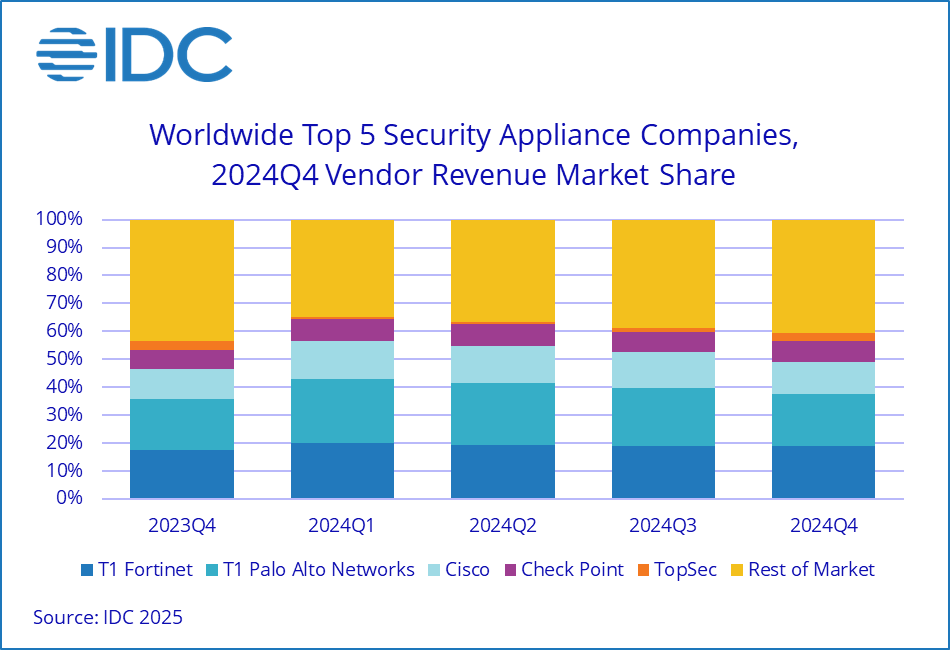
\includegraphics[width=0.8\textwidth]{Fortinet_Marktanteile.png}
	\caption{Marktanteil Fortinet}
	\label{fig:ER-Modell}
\end{figure}
https://my.idc.com/getdoc.jsp?containerId=prUS53243925


\begin{figure}[htbp]
	\centering
	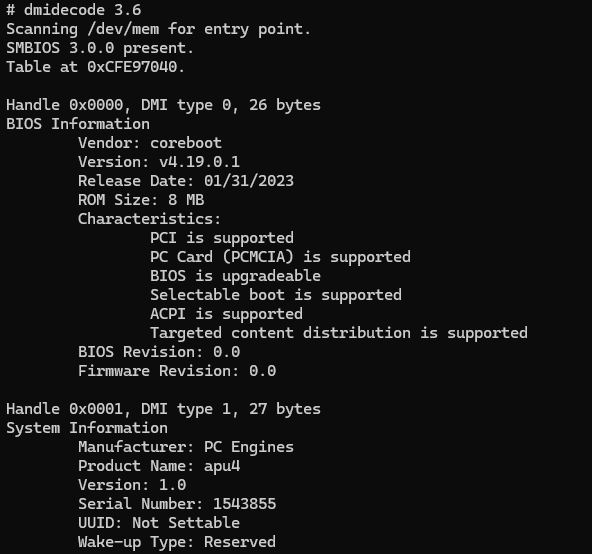
\includegraphics[width=0.8\textwidth]{opnsense-hardware.png}
	\caption{Die Hardwarekomponenten der Firewall.}
	\label{fig:hardware-apu4} % <-- SCHRITT 1: Marker setzen
\end{figure}

\begin{figure}[htbp]
	\centering
	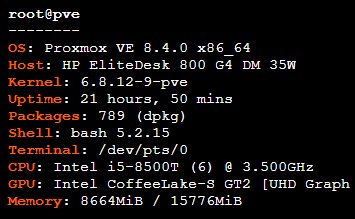
\includegraphics[width=0.8\textwidth]{proxmox-hardware.png}
	\caption{Die Hardwarekomponenten der ProxmoxVE-Umgebung.}
	\label{fig:hardware-prox} % <-- SCHRITT 1: Marker setzen
\end{figure}

\begin{figure}[htbp]
	\centering
	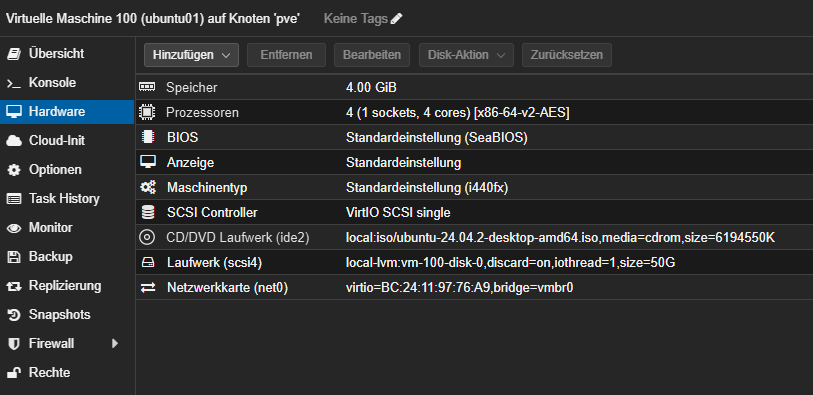
\includegraphics[width=0.8\textwidth]{ubuntu01-hardware.png}
	\caption{Zuweisung der Hardwareressourcen für Ubuntu-VMs}
	\label{fig:ubuntu-hardware} % <-- SCHRITT 1: Marker setzen
\end{figure}

\begin{figure}[htbp]
	\centering
	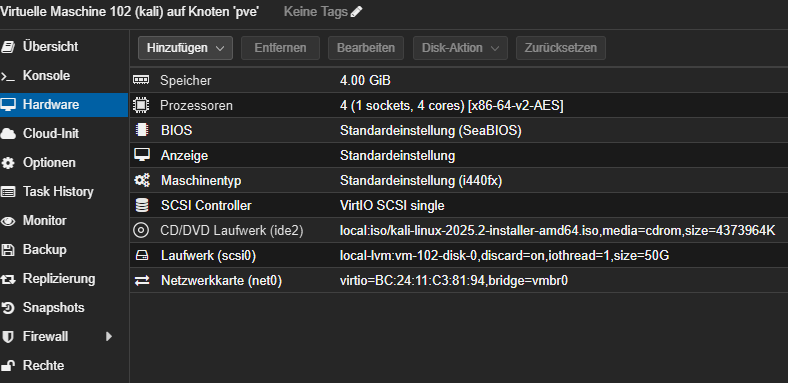
\includegraphics[width=0.8\textwidth]{kalivm-hardware.png}
	\caption{Zuweisung der Hardwareressourcen für Kali-Linux-VM}
	\label{fig:kali-hardware} % <-- SCHRITT 1: Marker setzen
\end{figure}

\begin{figure}[htbp]
	\centering
	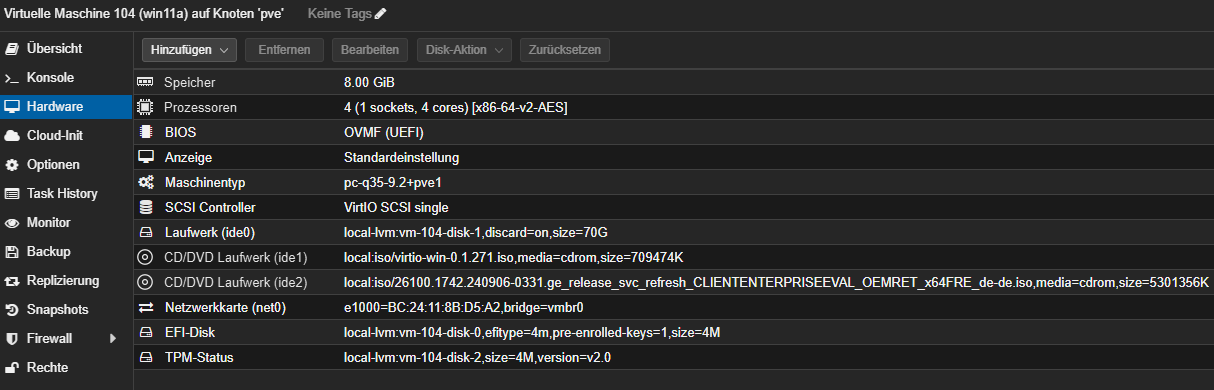
\includegraphics[width=0.8\textwidth]{win11-hardware.png}
	\caption{Zuweisung der Hardwareressourcen für Windows11-VM}
	\label{fig:win11-hardware} % <-- SCHRITT 1: Marker setzen
\end{figure}

\begin{figure}[htbp]
	\centering
	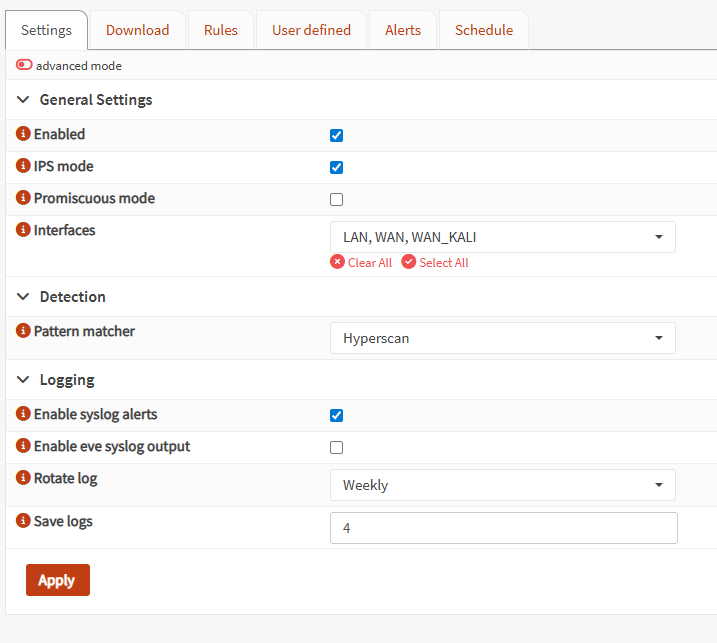
\includegraphics[width=0.8\textwidth]{IPSopnsense.png}
	\caption{Aktivierung des IDS und IPS}
	\label{fig:ipsopn1} % <-- SCHRITT 1: Marker setzen
\end{figure}

\begin{figure}[htbp]
	\centering
	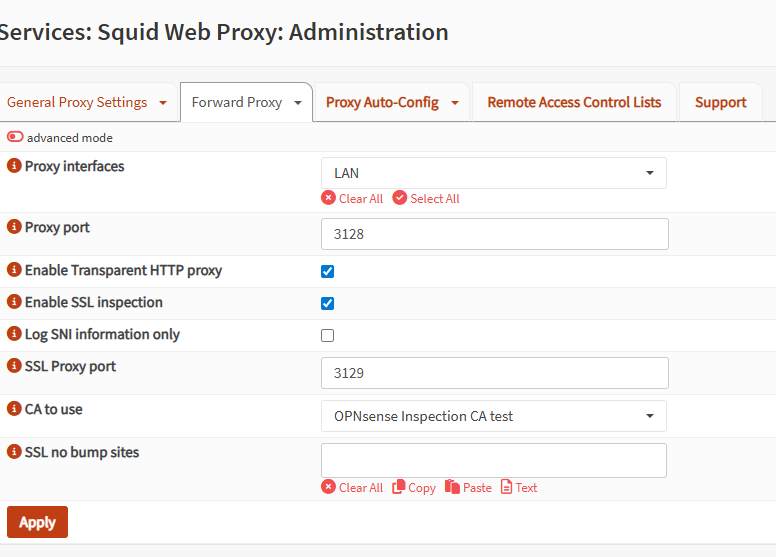
\includegraphics[width=0.8\textwidth]{squidproxy.png}
	\caption{Aktivierung des Squid Web Proxy mit SSL Inspection}
	\label{fig:squidproxy} % <-- SCHRITT 1: Marker setzen
\end{figure}

\begin{figure}[htbp]
	\centering
	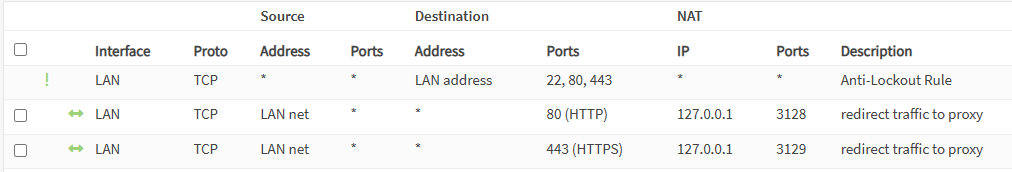
\includegraphics[width=0.8\textwidth]{proxyNAT.png}
	\caption{NAT Regeln zum Umleiten auf den Proxy}
	\label{fig:squidproxy} % <-- SCHRITT 1: Marker setzen
\end{figure}

\begin{figure}[htbp]
	\centering
	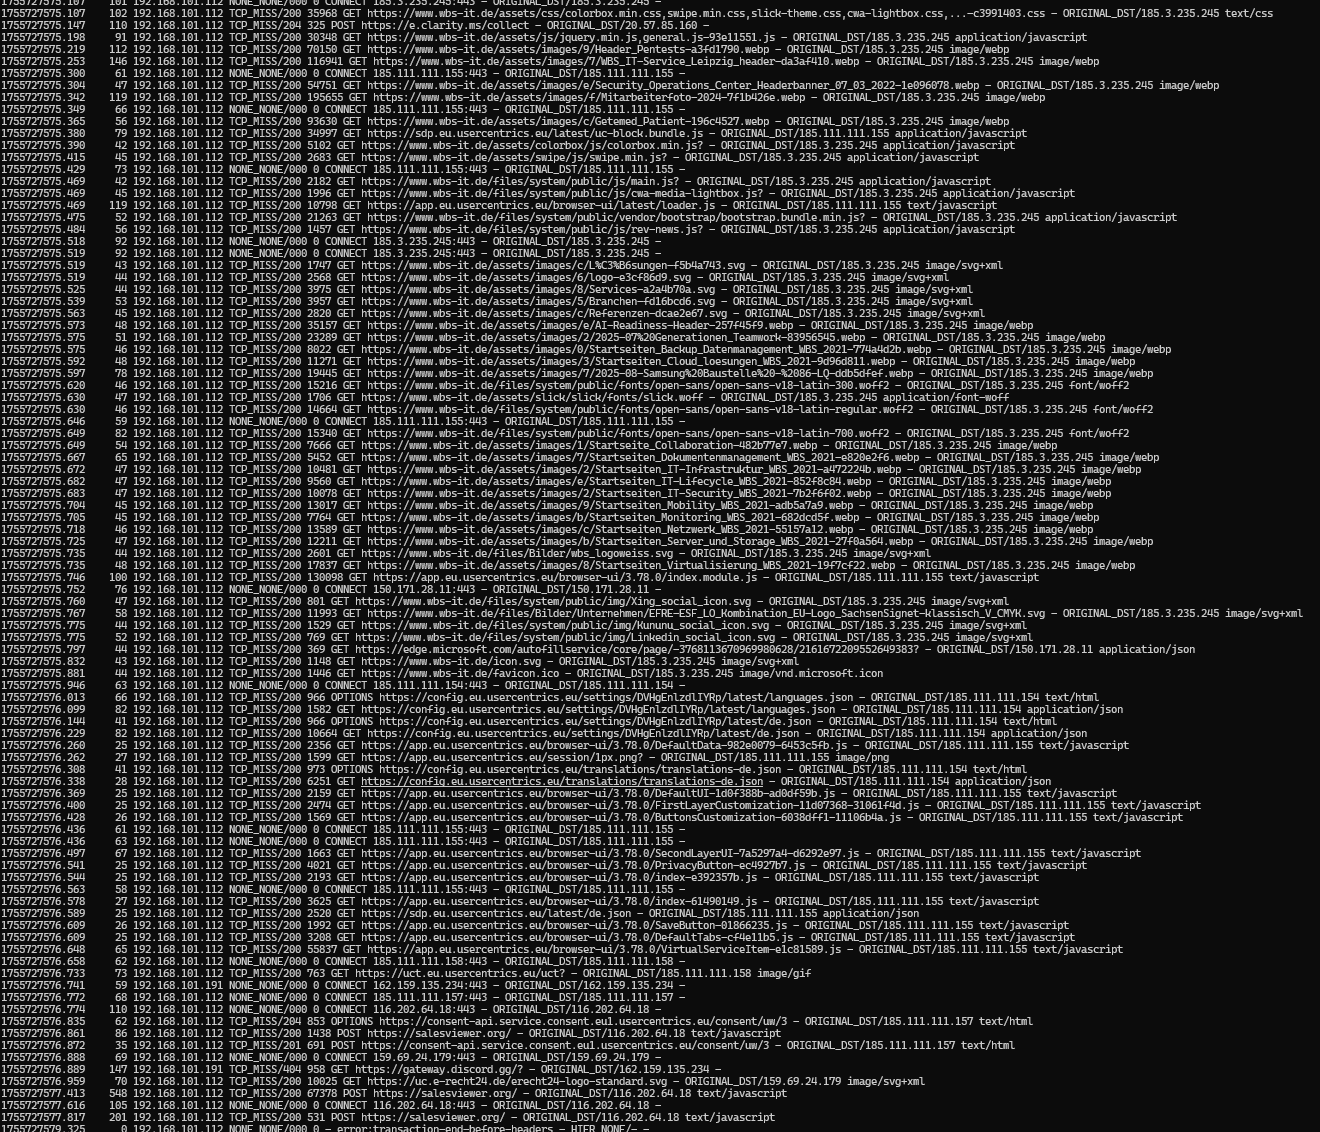
\includegraphics[width=0.8\textwidth]{squidproxy-log.png}
	\caption{Live Log Einträge des Web Proxy}
	\label{fig:proxylog} % <-- SCHRITT 1: Marker setzen
\end{figure}



	\end{thebibliography}
	\newpage
	
\end{document}



